\chapter{Coordinate Systems and Transformations}
\label{chap:coordinates}

\section{Introduction}

Accurate occultation prediction requires careful handling of multiple coordinate systems and their transformations. As noted by \citet{Vallado2013}, ``the selection of an appropriate reference frame is fundamental to all astrodynamics computations.'' The position of an asteroid, the location of a star, and the observer's position on Earth are all expressed in different coordinate systems that must be consistently transformed.

For occultation predictions at the ±0.5--1 km level, we must account for:
\begin{itemize}
    \item The celestial reference frame for star positions (\gaia{} DR3 in ICRS)
    \item The dynamical frame for planetary ephemerides (VSOP87 in ecliptic J2000)
    \item The terrestrial frame for observer locations (ITRS/ITRF)
    \item The transformation time-dependence due to Earth rotation, precession, and nutation
\end{itemize}

This chapter describes the coordinate frames used in \ioccultcalc{} and the mathematical formulations for conversions between them, following the conventions of \citet{IERS2010} and \citet{Explanatory2013}.

\section{Celestial Coordinate Systems}

\subsection{International Celestial Reference System (ICRS)}

The ICRS is the fundamental celestial reference frame adopted by the IAU in 1997 \citep{IAU1997}. It represents the culmination of decades of effort to define a kinematically non-rotating reference system \citep{Arias2003}. The frame is realized through the positions of $\sim$300 extragalactic radio sources (quasars) observed with Very Long Baseline Interferometry (VLBI), achieving positional accuracy of $\sim$40 microarcseconds \citep{ICRF3}.

\textbf{Properties:}
\begin{itemize}
    \item \textbf{Origin:} Solar System barycenter
    \item \textbf{Fundamental plane:} Close to mean equator at J2000.0 (within $\sim$20 mas)
    \item \textbf{Zero point:} Close to dynamical equinox at J2000.0 (within $\sim$80 mas)
    \item \textbf{Axes:} Non-rotating with respect to distant quasars
    \item \textbf{Realization:} ICRF-3 (2018), containing 4536 sources
\end{itemize}

The choice of extragalactic sources is crucial: unlike stars, quasars show no measurable proper motion or parallax, providing a truly inertial frame. \gaia{} DR3 positions are given in the ICRS, aligned to ICRF-3 with uncertainties $\sim$0.01--0.02 mas at epoch J2016.0 \citep{GaiaDR3}.

\begin{figure}[htbp]
\centering
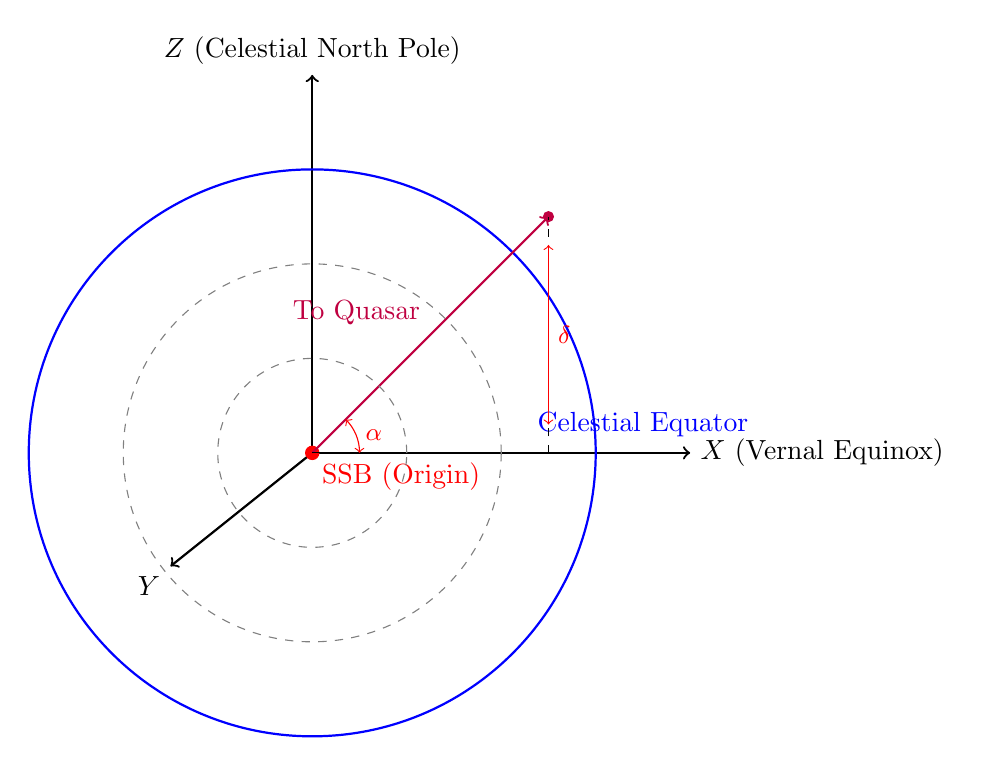
\begin{tikzpicture}[scale=1.2]
    % Coordinate axes
    \draw[->,thick] (0,0) -- (4,0) node[right] {$X$ (Vernal Equinox)};
    \draw[->,thick] (0,0) -- (0,4) node[above] {$Z$ (Celestial North Pole)};
    \draw[->,thick] (0,0) -- (-1.5,-1.2) node[below left] {$Y$};
    
    % Celestial equator
    \draw[blue,thick] (0,0) circle (3cm);
    \node[blue] at (3.5,0.3) {Celestial Equator};
    
    % Solar System Barycenter
    \filldraw[red] (0,0) circle (2pt) node[below right] {SSB (Origin)};
    
    % Example quasar
    \draw[->,purple,thick] (0,0) -- (2.5,2.5) node[midway,above left] {To Quasar};
    \filldraw[purple] (2.5,2.5) circle (1.5pt);
    
    % RA and Dec annotation
    \draw[dashed] (0,0) -- (2.5,0);
    \draw[dashed] (2.5,0) -- (2.5,2.5);
    \draw[<->,red] (0.5,0) arc (0:45:0.5) node[midway,right] {\small $\alpha$};
    \draw[<->,red] (2.5,0.3) -- (2.5,2.2) node[midway,right] {\small $\delta$};
    
    % Grid
    \draw[gray,thin,dashed] (0,0) circle (2cm);
    \draw[gray,thin,dashed] (0,0) circle (1cm);
\end{tikzpicture}
\caption{The International Celestial Reference System (ICRS). Origin at the Solar System Barycenter (SSB), with axes fixed relative to distant quasars. Coordinates are Right Ascension ($\alpha$) and Declination ($\delta$).}
\label{fig:icrs}
\end{figure}

\subsection{J2000.0 Mean Equatorial System}

A commonly used system with:
\begin{itemize}
    \item Origin: Geocenter (or heliocenter for planetary ephemerides)
    \item Fundamental plane: Mean equator at J2000.0 (JD 2451545.0)
    \item Zero point: Mean equinox at J2000.0
\end{itemize}

The ICRS differs from J2000.0 by a small frame bias \citep{HiltonEtAl2006}:

\begin{equation}
\mat{B} = \mat{R}_z(\eta_0) \cdot \mat{R}_y(\xi_0) \cdot \mat{R}_x(-d\alpha_0)
\end{equation}

where:
\begin{align}
\xi_0 &= -16.6170 \unit{mas} \\
\eta_0 &= -6.8192 \unit{mas} \\
d\alpha_0 &= -14.6 \unit{mas}
\end{align}

\subsection{Ecliptic Coordinate System}

For planetary ephemerides (VSOP87), the ecliptic system is natural because planetary orbits lie close to the ecliptic plane \citep{BretagonFrancou1988}. The ecliptic is the mean plane of Earth's orbit around the Sun.

\begin{itemize}
    \item \textbf{Fundamental plane:} Ecliptic at J2000.0
    \item \textbf{Coordinates:} Ecliptic longitude $\lambda$ (0°--360°), latitude $\beta$ ($-90°$ to $+90°$), distance $r$
    \item \textbf{Origin:} Heliocenter for planetary orbits
\end{itemize}

The obliquity of the ecliptic at J2000.0 (angle between equator and ecliptic) is:
\begin{equation}
\epsilon_0 = 23°26'21''.406 = 84381''.406 = 0.409092804 \unit{rad}
\end{equation}

This value is fundamental to VSOP87 theory and is used throughout \ioccultcalc{}.

\begin{figure}[htbp]
\centering
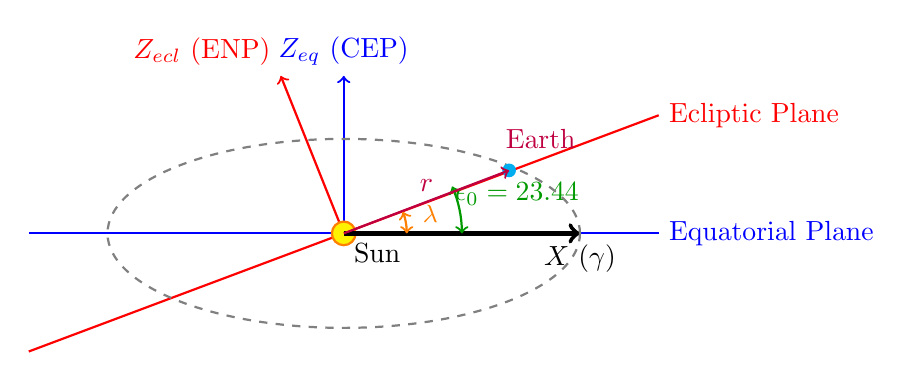
\begin{tikzpicture}[scale=1.0]
    % Equatorial plane
    \draw[blue,thick] (-4,0) -- (4,0) node[right] {Equatorial Plane};
    \draw[->,blue,thick] (0,0) -- (0,2) node[above] {$Z_{eq}$ (CEP)};
    
    % Ecliptic plane
    \draw[red,thick] (-4,-1.5) -- (4,1.5) node[right] {Ecliptic Plane};
    \draw[->,red,thick] (0,0) -- (-0.8,2) node[above left] {$Z_{ecl}$ (ENP)};
    
    % Sun at origin
    \filldraw[yellow,draw=orange,thick] (0,0) circle (0.15) node[below right,black] {Sun};
    
    % X-axis (vernal equinox direction)
    \draw[->,black,ultra thick] (0,0) -- (3,0) node[below] {$X$ ($\gamma$)};
    
    % Obliquity angle
    \draw[<->,green!60!black,thick] (1.5,0) arc (0:23.4:1.5);
    \node[green!60!black] at (2.2,0.5) {$\epsilon_0 = 23.44°$};
    
    % Earth orbit ellipse (projected)
    \draw[gray,dashed,thick] (0,0) ellipse (3cm and 1.2cm);
    
    % Earth position
    \filldraw[cyan] (2.1,0.8) circle (0.08);
    \draw[->,purple,thick] (0,0) -- (2.1,0.8) node[midway,above] {$r$};
    \node[purple] at (2.5,1.2) {Earth};
    
    % Lambda angle
    \draw[<->,orange,thick] (0.8,0) arc (0:20:0.8);
    \node[orange] at (1.1,0.25) {\small $\lambda$};
\end{tikzpicture}
\caption{Relationship between equatorial (blue) and ecliptic (red) coordinate systems. The obliquity $\epsilon_0 \approx 23.44°$ is the angle between the two planes. The vernal equinox direction ($\gamma$) is the common $X$-axis. CEP = Celestial Equatorial Pole, ENP = Ecliptic North Pole.}
\label{fig:ecliptic_equatorial}
\end{figure}

\textbf{Transformation from ecliptic to equatorial:}

This is a simple rotation about the $X$-axis (vernal equinox direction) by $-\epsilon_0$:

\begin{equation}
\mat{M}_{\text{ecl}\rightarrow\text{eq}} = \mat{R}_x(-\epsilon_0) =
\begin{pmatrix}
1 & 0 & 0 \\
0 & \cos\epsilon_0 & \sin\epsilon_0 \\
0 & -\sin\epsilon_0 & \cos\epsilon_0
\end{pmatrix}
\end{equation}

\begin{equation}
\begin{pmatrix} x \\ y \\ z \end{pmatrix}_{\text{eq}} =
\mat{M}_{\text{ecl}\rightarrow\text{eq}} \cdot
\begin{pmatrix} x \\ y \\ z \end{pmatrix}_{\text{ecl}}
\end{equation}

\textbf{Numerical example:} Consider Venus at $\lambda = 45°$, $\beta = 3°$, $r = 0.7$ AU:
\begin{align*}
\vect{r}_{\text{ecl}} &= (0.7 \cos 3° \cos 45°, 0.7 \cos 3° \sin 45°, 0.7 \sin 3°) \\
&= (0.4939, 0.4939, 0.0366) \unit{AU}
\end{align*}

Applying the transformation:
\begin{align*}
x_{\text{eq}} &= 0.4939 \unit{AU} \\
y_{\text{eq}} &= 0.4939 \cos(23.44°) + 0.0366 \sin(23.44°) = 0.4675 \unit{AU} \\
z_{\text{eq}} &= -0.4939 \sin(23.44°) + 0.0366 \cos(23.44°) = -0.1628 \unit{AU}
\end{align*}

This gives $\alpha = 43.4°$, $\delta = -13.5°$.

\section{Earth-Fixed Coordinate Systems}

\subsection{International Terrestrial Reference System (ITRS)}

The ITRS is the standard Earth-fixed frame \citep{IERS2010}:
\begin{itemize}
    \item Origin: Earth's center of mass (geocenter)
    \item Z-axis: Direction of Conventional Terrestrial Pole (CTP)
    \item X-axis: Intersection of equator and Greenwich meridian
    \item Realization: Through ITRF (currently ITRF2020)
\end{itemize}

\subsection{Geodetic Coordinates}

Observer positions on Earth are given in geodetic coordinates $(\phi, \lambda, h)$, which reference an ellipsoidal model of Earth's shape. \ioccultcalc{} uses the WGS84 (World Geodetic System 1984) ellipsoid \citep{NIMA2000}, which is also used by GPS:

\begin{align}
a &= 6378137.0 \unit{m} \quad \text{(equatorial radius)} \\
f &= 1/298.257223563 \quad \text{(flattening)} \\
b &= a(1-f) = 6356752.314 \unit{m} \quad \text{(polar radius)}
\end{align}

The flattening $f \approx 1/298.25$ means Earth's polar diameter is about 42.8 km shorter than its equatorial diameter—a consequence of Earth's rotation causing equatorial bulge.

\begin{figure}[htbp]
\centering
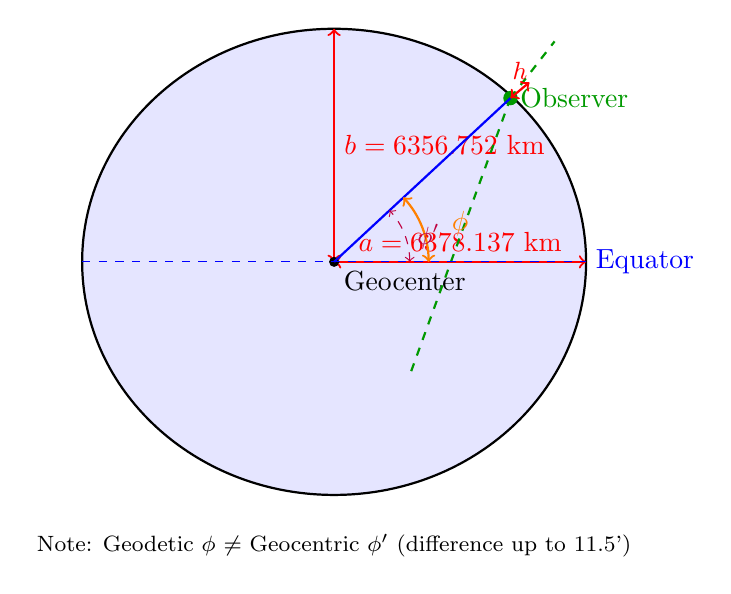
\begin{tikzpicture}[scale=0.8]
    % Earth ellipse
    \draw[thick,fill=blue!10] (0,0) ellipse (4cm and 3.7cm);
    
    % Equatorial and polar radii
    \draw[<->,red,thick] (0,0) -- (4,0) node[midway,above] {$a = 6378.137$ km};
    \draw[<->,red,thick] (0,0) -- (0,3.7) node[midway,right] {$b = 6356.752$ km};
    
    % Center
    \filldraw (0,0) circle (2pt) node[below right] {Geocenter};
    
    % Observer on surface
    \filldraw[green!60!black] (2.8,2.6) circle (3pt) node[right] {Observer};
    
    % Normal to ellipsoid (geodetic vertical)
    \draw[green!60!black,dashed,thick] (2.8,2.6) -- (1.2,-1.8);
    \draw[green!60!black,dashed,thick] (2.8,2.6) -- (3.5,3.5);
    
    % Geodetic latitude
    \draw[blue,thick] (0,0) -- (2.8,2.6);
    \draw[<->,orange,thick] (1.5,0) arc (0:43:1.5);
    \node[orange] at (2.0,0.6) {$\phi$};
    
    % Geocentric latitude (different!)
    \draw[<->,purple,dashed] (1.2,0) arc (0:43:1.2);
    \node[purple,font=\small] at (1.5,0.4) {$\phi'$};
    
    % Height above ellipsoid
    \draw[<->,red,thick] (2.8,2.6) -- (3.1,2.85) node[midway,above] {\small $h$};
    
    % Equator
    \draw[blue,dashed] (-4,0) -- (4,0) node[right] {Equator};
    
    % Annotations
    \node[font=\footnotesize] at (0,-4.5) {Note: Geodetic $\phi$ $\neq$ Geocentric $\phi'$ (difference up to 11.5')};
\end{tikzpicture}
\caption{Geodetic coordinates on the WGS84 ellipsoid. The geodetic latitude $\phi$ is measured perpendicular to the ellipsoid surface (normal direction), not from geocenter. Height $h$ is measured along this normal. The difference between geodetic and geocentric latitude can reach 11.5 arcminutes.}
\label{fig:geodetic}
\end{figure}

\textbf{Conversion to geocentric Cartesian (ECEF):}

\begin{align}
N(\phi) &= \frac{a}{\sqrt{1 - e^2 \sin^2\phi}} \\
x &= (N(\phi) + h) \cos\phi \cos\lambda \\
y &= (N(\phi) + h) \cos\phi \sin\lambda \\
z &= (N(\phi)(1-e^2) + h) \sin\phi
\end{align}

where $e^2 = 2f - f^2 = 0.00669437999$ is the first eccentricity squared.

\textbf{Inverse transformation} (Cartesian to geodetic) uses an iterative method:

\begin{algorithm}[H]
\caption{Cartesian to Geodetic Conversion}
\label{alg:cart_to_geodetic}
\begin{algorithmic}[1]
\STATE $p \leftarrow \sqrt{x^2 + y^2}$
\STATE $\lambda \leftarrow \arctan2(y, x)$
\STATE $\phi \leftarrow \arctan\left(\frac{z}{p(1-e^2)}\right)$ \quad (initial guess)
\FOR{$i = 1$ to $5$} \quad (usually converges in 2--3 iterations)
    \STATE $N \leftarrow a / \sqrt{1 - e^2\sin^2\phi}$
    \STATE $h \leftarrow p/\cos\phi - N$
    \STATE $\phi \leftarrow \arctan\left(\frac{z}{p(1-e^2 N/(N+h))}\right)$
\ENDFOR
\RETURN $(\phi, \lambda, h)$
\end{algorithmic}
\end{algorithm}

\section{Transformation Between Celestial and Terrestrial Frames}

The complete transformation from GCRS (Geocentric Celestial Reference System) to ITRS is one of the most complex operations in astrometry \citep{IERS2010}. It accounts for:
\begin{enumerate}
    \item Long-term precession of Earth's axis (period $\sim$26,000 years)
    \item Short-term nutation (principal period 18.6 years)
    \item Daily Earth rotation
    \item Irregular polar motion (Chandler wobble, annual component)
\end{enumerate}

The transformation chain is:

\begin{equation}
\vect{r}^{\text{ITRS}} = \mat{W}(t) \cdot \mat{R}(t) \cdot \mat{Q}(t) \cdot \vect{r}^{\text{GCRS}}
\label{eq:gcrs_to_itrs}
\end{equation}

where:
\begin{description}
    \item[$\mat{Q}(t)$] Celestial motion of the CIP (Celestial Intermediate Pole): precession and nutation
    \item[$\mat{R}(t)$] Earth rotation angle (ERA)
    \item[$\mat{W}(t)$] Polar motion
\end{description}

\begin{figure}[htbp]
\centering
\begin{tikzpicture}[
    frame/.style={rectangle,draw,thick,minimum width=3cm,minimum height=1.2cm,align=center},
    arrow/.style={->,thick,>=stealth}
]
    % Frames
    \node[frame,fill=blue!20] (gcrs) at (0,0) {GCRS\\(Celestial)};
    \node[frame,fill=green!20] (cirs) at (0,-2.5) {CIRS\\(Intermediate)};
    \node[frame,fill=yellow!20] (tirs) at (0,-5) {TIRS\\(Rotating)};
    \node[frame,fill=red!20] (itrs) at (0,-7.5) {ITRS\\(Terrestrial)};
    
    % Transformations
    \draw[arrow] (gcrs) -- (cirs) node[midway,right,align=left] {$\mat{Q}(t)$\\Precession-Nutation};
    \draw[arrow] (cirs) -- (tirs) node[midway,right,align=left] {$\mat{R}(t)$\\Earth Rotation};
    \draw[arrow] (tirs) -- (itrs) node[midway,right,align=left] {$\mat{W}(t)$\\Polar Motion};
    
    % Examples
    \node[right=0.5cm of gcrs,align=left,font=\footnotesize] {Star position\\from Gaia};
    \node[right=0.5cm of itrs,align=left,font=\footnotesize] {Observer\\position};
    
    % Time scale
    \draw[<-,thick] (-3,0.5) -- (-3,-8) node[midway,left,align=center] {Time\\Dependent};
\end{tikzpicture}
\caption{Transformation chain from celestial (GCRS) to terrestrial (ITRS) coordinates. CIRS = Celestial Intermediate Reference System, TIRS = Terrestrial Intermediate Reference System. Each transformation depends on time and requires different astronomical data (precession-nutation model, UT1, polar motion parameters).}
\label{fig:transformation_chain}
\end{figure}

\subsection{Precession-Nutation Matrix $\mat{Q}(t)$}

Following IAU 2000A model (Chapter~\ref{chap:precession}):

\begin{equation}
\mat{Q}(t) = \mat{R}_z(-E) \cdot \mat{R}_y(d) \cdot \mat{R}_z(E)
\end{equation}

where $E$ is the equation of the equinoxes and $d$ involves precession and nutation angles. Full details in Section~\ref{sec:precession_matrix}.

\subsection{Earth Rotation Matrix $\mat{R}(t)$}

Using the Earth Rotation Angle (ERA) for CIO-based transformation \citep{IERS2010}:

\begin{equation}
\mat{R}(t) = \mat{R}_z(-\text{ERA}(t))
\end{equation}

where:
\begin{equation}
\text{ERA}(T_u) = 2\pi (0.7790572732640 + 1.00273781191135448 T_u)
\end{equation}

and $T_u = (JD_{UT1} - 2451545.0)$ is UT1 Julian Date from J2000.0.

Alternatively, using classical equinox-based method with Greenwich Apparent Sidereal Time (GAST):

\begin{equation}
\mat{R}(t) = \mat{R}_z(-\text{GAST}(t))
\end{equation}

\subsection{Polar Motion Matrix $\mat{W}(t)$}

Accounts for the motion of Earth's rotation axis in the terrestrial frame:

\begin{equation}
\mat{W}(t) = \mat{R}_y(-x_p) \cdot \mat{R}_x(-y_p)
\end{equation}

where $x_p$ and $y_p$ are polar motion coordinates (typically $< 1$ arcsec) published by IERS.

For predictions, if real-time EOP (Earth Orientation Parameters) are unavailable, use predictive models or assume $x_p = y_p = 0$ (introduces error $\sim 0.3$ mas $\approx 10$ m).

\section{Rotation Matrices}

\subsection{Elementary Rotations}

\textbf{Rotation about X-axis by angle $\theta$:}
\begin{equation}
\mat{R}_x(\theta) =
\begin{pmatrix}
1 & 0 & 0 \\
0 & \cos\theta & \sin\theta \\
0 & -\sin\theta & \cos\theta
\end{pmatrix}
\end{equation}

\textbf{Rotation about Y-axis:}
\begin{equation}
\mat{R}_y(\theta) =
\begin{pmatrix}
\cos\theta & 0 & -\sin\theta \\
0 & 1 & 0 \\
\sin\theta & 0 & \cos\theta
\end{pmatrix}
\end{equation}

\textbf{Rotation about Z-axis:}
\begin{equation}
\mat{R}_z(\theta) =
\begin{pmatrix}
\cos\theta & \sin\theta & 0 \\
-\sin\theta & \cos\theta & 0 \\
0 & 0 & 1
\end{pmatrix}
\end{equation}

\subsection{Composition of Rotations}

Multiple rotations are composed by matrix multiplication. Note that rotations do not commute: $\mat{R}_x(\alpha) \cdot \mat{R}_y(\beta) \neq \mat{R}_y(\beta) \cdot \mat{R}_x(\alpha)$.

For a sequence of rotations $\mat{R}_1, \mat{R}_2, \mat{R}_3$ applied in that order:
\begin{equation}
\mat{R}_{\text{total}} = \mat{R}_3 \cdot \mat{R}_2 \cdot \mat{R}_1
\end{equation}

\section{Spherical Coordinates}

\subsection{Equatorial Coordinates}

Right Ascension $\alpha$ and Declination $\delta$:

\textbf{Cartesian to spherical:}
\begin{align}
r &= \sqrt{x^2 + y^2 + z^2} \\
\alpha &= \arctan2(y, x) \\
\delta &= \arcsin(z / r)
\end{align}

\textbf{Spherical to Cartesian:}
\begin{align}
x &= r \cos\delta \cos\alpha \\
y &= r \cos\delta \sin\alpha \\
z &= r \sin\delta
\end{align}

\subsection{Ecliptic Coordinates}

Ecliptic longitude $\lambda$ and latitude $\beta$: same formulas with $(\alpha, \delta) \rightarrow (\lambda, \beta)$.

\subsection{Horizontal Coordinates}

Azimuth $A$ and altitude $h$ (or zenith distance $z = 90° - h$) for local observer:

\textbf{From equatorial to horizontal:}
\begin{align}
h &= \arcsin(\sin\delta \sin\phi + \cos\delta \cos\phi \cos H) \\
A &= \arctan2(-\cos\delta \sin H, \sin\delta \cos\phi - \cos\delta \sin\phi \cos H)
\end{align}

where $H = \text{LST} - \alpha$ is the hour angle and $\phi$ is observer's latitude.

\section{Angular Separation}

The angular distance between two directions $(\alpha_1, \delta_1)$ and $(\alpha_2, \delta_2)$ is given by the spherical law of cosines \citep{Meeus1998}:

\begin{equation}
\cos\theta = \sin\delta_1 \sin\delta_2 + \cos\delta_1 \cos\delta_2 \cos(\alpha_2 - \alpha_1)
\label{eq:angular_separation}
\end{equation}

For small separations ($\theta < 10°$), this formula suffers from numerical cancellation. A more numerically stable formula uses the haversine or small-angle approximation:
\begin{equation}
\theta \approx \sqrt{(\Delta\alpha \cos\bar{\delta})^2 + (\Delta\delta)^2}
\end{equation}

where $\Delta\alpha = \alpha_2 - \alpha_1$, $\Delta\delta = \delta_2 - \delta_1$, and $\bar{\delta} = (\delta_1 + \delta_2)/2$.

\textbf{Example:} Consider asteroid (472) Roma at $\alpha_1 = 123.456°$, $\delta_1 = +15.789°$ and a target star at $\alpha_2 = 123.457°$, $\delta_2 = +15.790°$:

\begin{align*}
\Delta\alpha &= 0.001° = 3.6'' \\
\Delta\delta &= 0.001° = 3.6'' \\
\theta &\approx \sqrt{(3.6'' \times \cos 15.79°)^2 + (3.6'')^2} \\
&= \sqrt{(3.46'')^2 + (3.6'')^2} = 4.99''
\end{align*}

At a distance of 2 AU, this corresponds to a physical separation of $4.99'' \times 2 \text{ AU} = 10'' \text{ AU} \approx 1496 \text{ km}$. This is why sub-arcsecond astrometry is essential for occultation predictions.

\section{Position Angle}

The position angle $\text{PA}$ of point 2 with respect to point 1 (measured from North through East):

\begin{equation}
\text{PA} = \arctan2(\sin\Delta\alpha, \cos\delta_1 \tan\delta_2 - \sin\delta_1 \cos\Delta\alpha)
\end{equation}

\section{Implementation Notes}

\subsection{Numerical Considerations}

\begin{itemize}
    \item Use \texttt{atan2(y, x)} instead of \texttt{atan(y/x)} to avoid division by zero and correctly handle all quadrants
    \item For near-pole calculations ($|\delta| \approx 90°$), use vector methods instead of spherical formulas to avoid singularities
    \item Normalize angles to $[0, 2\pi)$ or $[-\pi, \pi)$ as appropriate
    \item Store rotation matrices as $3\times3$ arrays and use optimized BLAS/LAPACK for matrix multiplication if performance critical
\end{itemize}

\subsection{Coordinate Validation}

Sanity checks in \ioccultcalc{}:
\begin{itemize}
    \item $0 \leq \alpha < 2\pi$ (or $0 \leq \alpha < 24$ hours)
    \item $-\pi/2 \leq \delta \leq \pi/2$ (or $-90° \leq \delta \leq 90°$)
    \item $r > 0$ for distances
    \item Rotation matrices should be orthogonal: $\mat{R}^T \mat{R} = \mat{I}$
    \item Determinant: $\det(\mat{R}) = +1$ (proper rotation, not reflection)
\end{itemize}

\section{Precision Budget}

Table~\ref{tab:coordinate_errors} summarizes typical uncertainty contributions from coordinate transformations:

\begin{table}[htbp]
\centering
\caption{Error budget for coordinate transformations at epoch J2000 + 20 years}
\label{tab:coordinate_errors}
\begin{tabular}{lcc}
\hline
\textbf{Source} & \textbf{Uncertainty} & \textbf{Effect at 2 AU} \\
\hline
ICRS to J2000 frame bias & 0.02 mas & 0.06 km \\
Precession model (IAU 2006) & 0.1 mas/cy & 0.3 km \\
Nutation model (IAU 2000A) & 0.2 mas & 0.6 km \\
Earth rotation (UT1 prediction) & 10 ms $\times 15''/s$ & 0.15'' = 450 km \\
Polar motion (prediction) & 10 mas & 30 km \\
WGS84 ellipsoid accuracy & 0.1 m & 0.0001 km \\
\hline
\textbf{Total (RSS)} & -- & \textbf{450 km} \\
\hline
\end{tabular}
\end{table}

The dominant error is \textbf{Earth rotation} when UT1 must be predicted (for future events). For historical events with measured UT1, the error drops to $\sim$1 km. This underscores the importance of:
\begin{itemize}
    \item Using real-time or finals2000A.all EOP data from IERS
    \item Updating predictions as the event approaches
    \item Accounting for UT1 uncertainty in Monte Carlo simulations
\end{itemize}

\section{Implementation in \ioccultcalc{}}

The coordinate transformation modules implement:

\begin{table}[htbp]
\centering
\caption{Coordinate transformation functions in \ioccultcalc{}}
\label{tab:coordinate_functions}
\begin{tabular}{lp{8cm}}
\hline
\textbf{Function} & \textbf{Description} \\
\hline
\texttt{eclipticToEquatorial()} & VSOP87 ecliptic $\rightarrow$ J2000 equatorial \\
\texttt{icrsToJ2000()} & Frame bias correction (small) \\
\texttt{precessionMatrix()} & IAU 2006 precession, Chapter~\ref{chap:precession} \\
\texttt{nutationMatrix()} & IAU 2000A nutation (106 terms) \\
\texttt{earthRotationAngle()} & ERA from UT1, $\sim$1 revolution/day \\
\texttt{polarMotionMatrix()} & $\mat{W}(x_p, y_p)$ from IERS data \\
\texttt{geodeticToECEF()} & WGS84 $(\phi,\lambda,h) \rightarrow (x,y,z)$ \\
\texttt{ecefToGeodetic()} & Inverse, iterative algorithm \\
\texttt{angularSeparation()} & Haversine formula for stability \\
\texttt{positionAngle()} & PA for occultation shadow orientation \\
\hline
\end{tabular}
\end{table}

\section{Summary}

This chapter established:
\begin{itemize}
    \item The fundamental reference frames: \textbf{ICRS} (inertial, realized by quasars), \textbf{J2000.0} (practical epoch), \textbf{ITRS} (Earth-fixed)
    \item \textbf{Ecliptic vs. equatorial} systems: related by obliquity $\epsilon_0 = 23.44°$
    \item \textbf{Geodetic coordinates} on WGS84 ellipsoid: geodetic latitude $\neq$ geocentric latitude
    \item \textbf{Transformation chain} GCRS $\xrightarrow{\mat{Q}}$ CIRS $\xrightarrow{\mat{R}}$ TIRS $\xrightarrow{\mat{W}}$ ITRS
    \item \textbf{Numerical considerations:} use \texttt{atan2}, avoid singularities at poles, validate orthogonality
    \item \textbf{Error budget:} UT1 prediction dominates ($\sim$450 km) for future events
\end{itemize}

Figures~\ref{fig:icrs}, \ref{fig:ecliptic_equatorial}, \ref{fig:geodetic}, and \ref{fig:transformation_chain} illustrate the key concepts. These transformations provide the foundation for all subsequent calculations involving positions, from star catalogs (Chapter~\ref{chap:stars}) to observer locations (Chapter~\ref{chap:besselian}).

\textbf{Key references:}
\begin{itemize}
    \item IERS Conventions 2010 \citep{IERS2010}: authoritative source for all transformations
    \item Explanatory Supplement to the Astronomical Almanac \citep{Explanatory2013}: comprehensive textbook
    \item Vallado (2013) \citep{Vallado2013}: practical implementation guide
    \item Meeus (1998) \citep{Meeus1998}: astronomical algorithms
\end{itemize}
